\chapter{Theory Background}
\section{Introduction}
Cryptanalysis is the technique of extracting useful information about the key by observing the plaintext and cipher text using cryptanalysis try to break the secrecy provided by the cipher. There is no fixed method for cryptanalysis and every cipher is a different challenge to the attacker and hence demands different insight to attack\cite{jha2011cryptanalysis},The study of cipher text in an attempt to restore the message to plaintext is known as cryptanalysis. Cryptanalysis is equally mathematically challenging and complex as cryptography. Because of the complexity involved with cryptanalysis work this document is only focused on the basic techniques needed to decipher monoalphabetic encryption ciphers and cryptograms\cite{smith2001basic}.
In this chapter, explained the history of cryptanalysis, the technology of cryptanalysis, transposition cipher, substitution cipher and description genetics algorithm (GA).

\section{Cryptanalysis}
Cryptanalysis is the technique of deriving the original
message from the ciphertext without any prior knowledge of
secret key or derivation of key from the ciphertext. A general
technique for cryptanalysis, applicable to all cryptographic
algorithms is to try all the possible keys until the correct key
is matched, it is known as exhaustive key search. With every
passing day, the computing ability of hardware is increasing
manifold; therefore it becomes necessary to use long keys for
avoiding exhaustive key search \cite{bokhari2012cryptanalysis} and till today, many cryptanalytic attacks are developed based on these. Each variant of these have different methods to find distinguisher and
based on the distinguisher \cite{khurana2015variants}.

\begin{figure}[h]
	\centering
	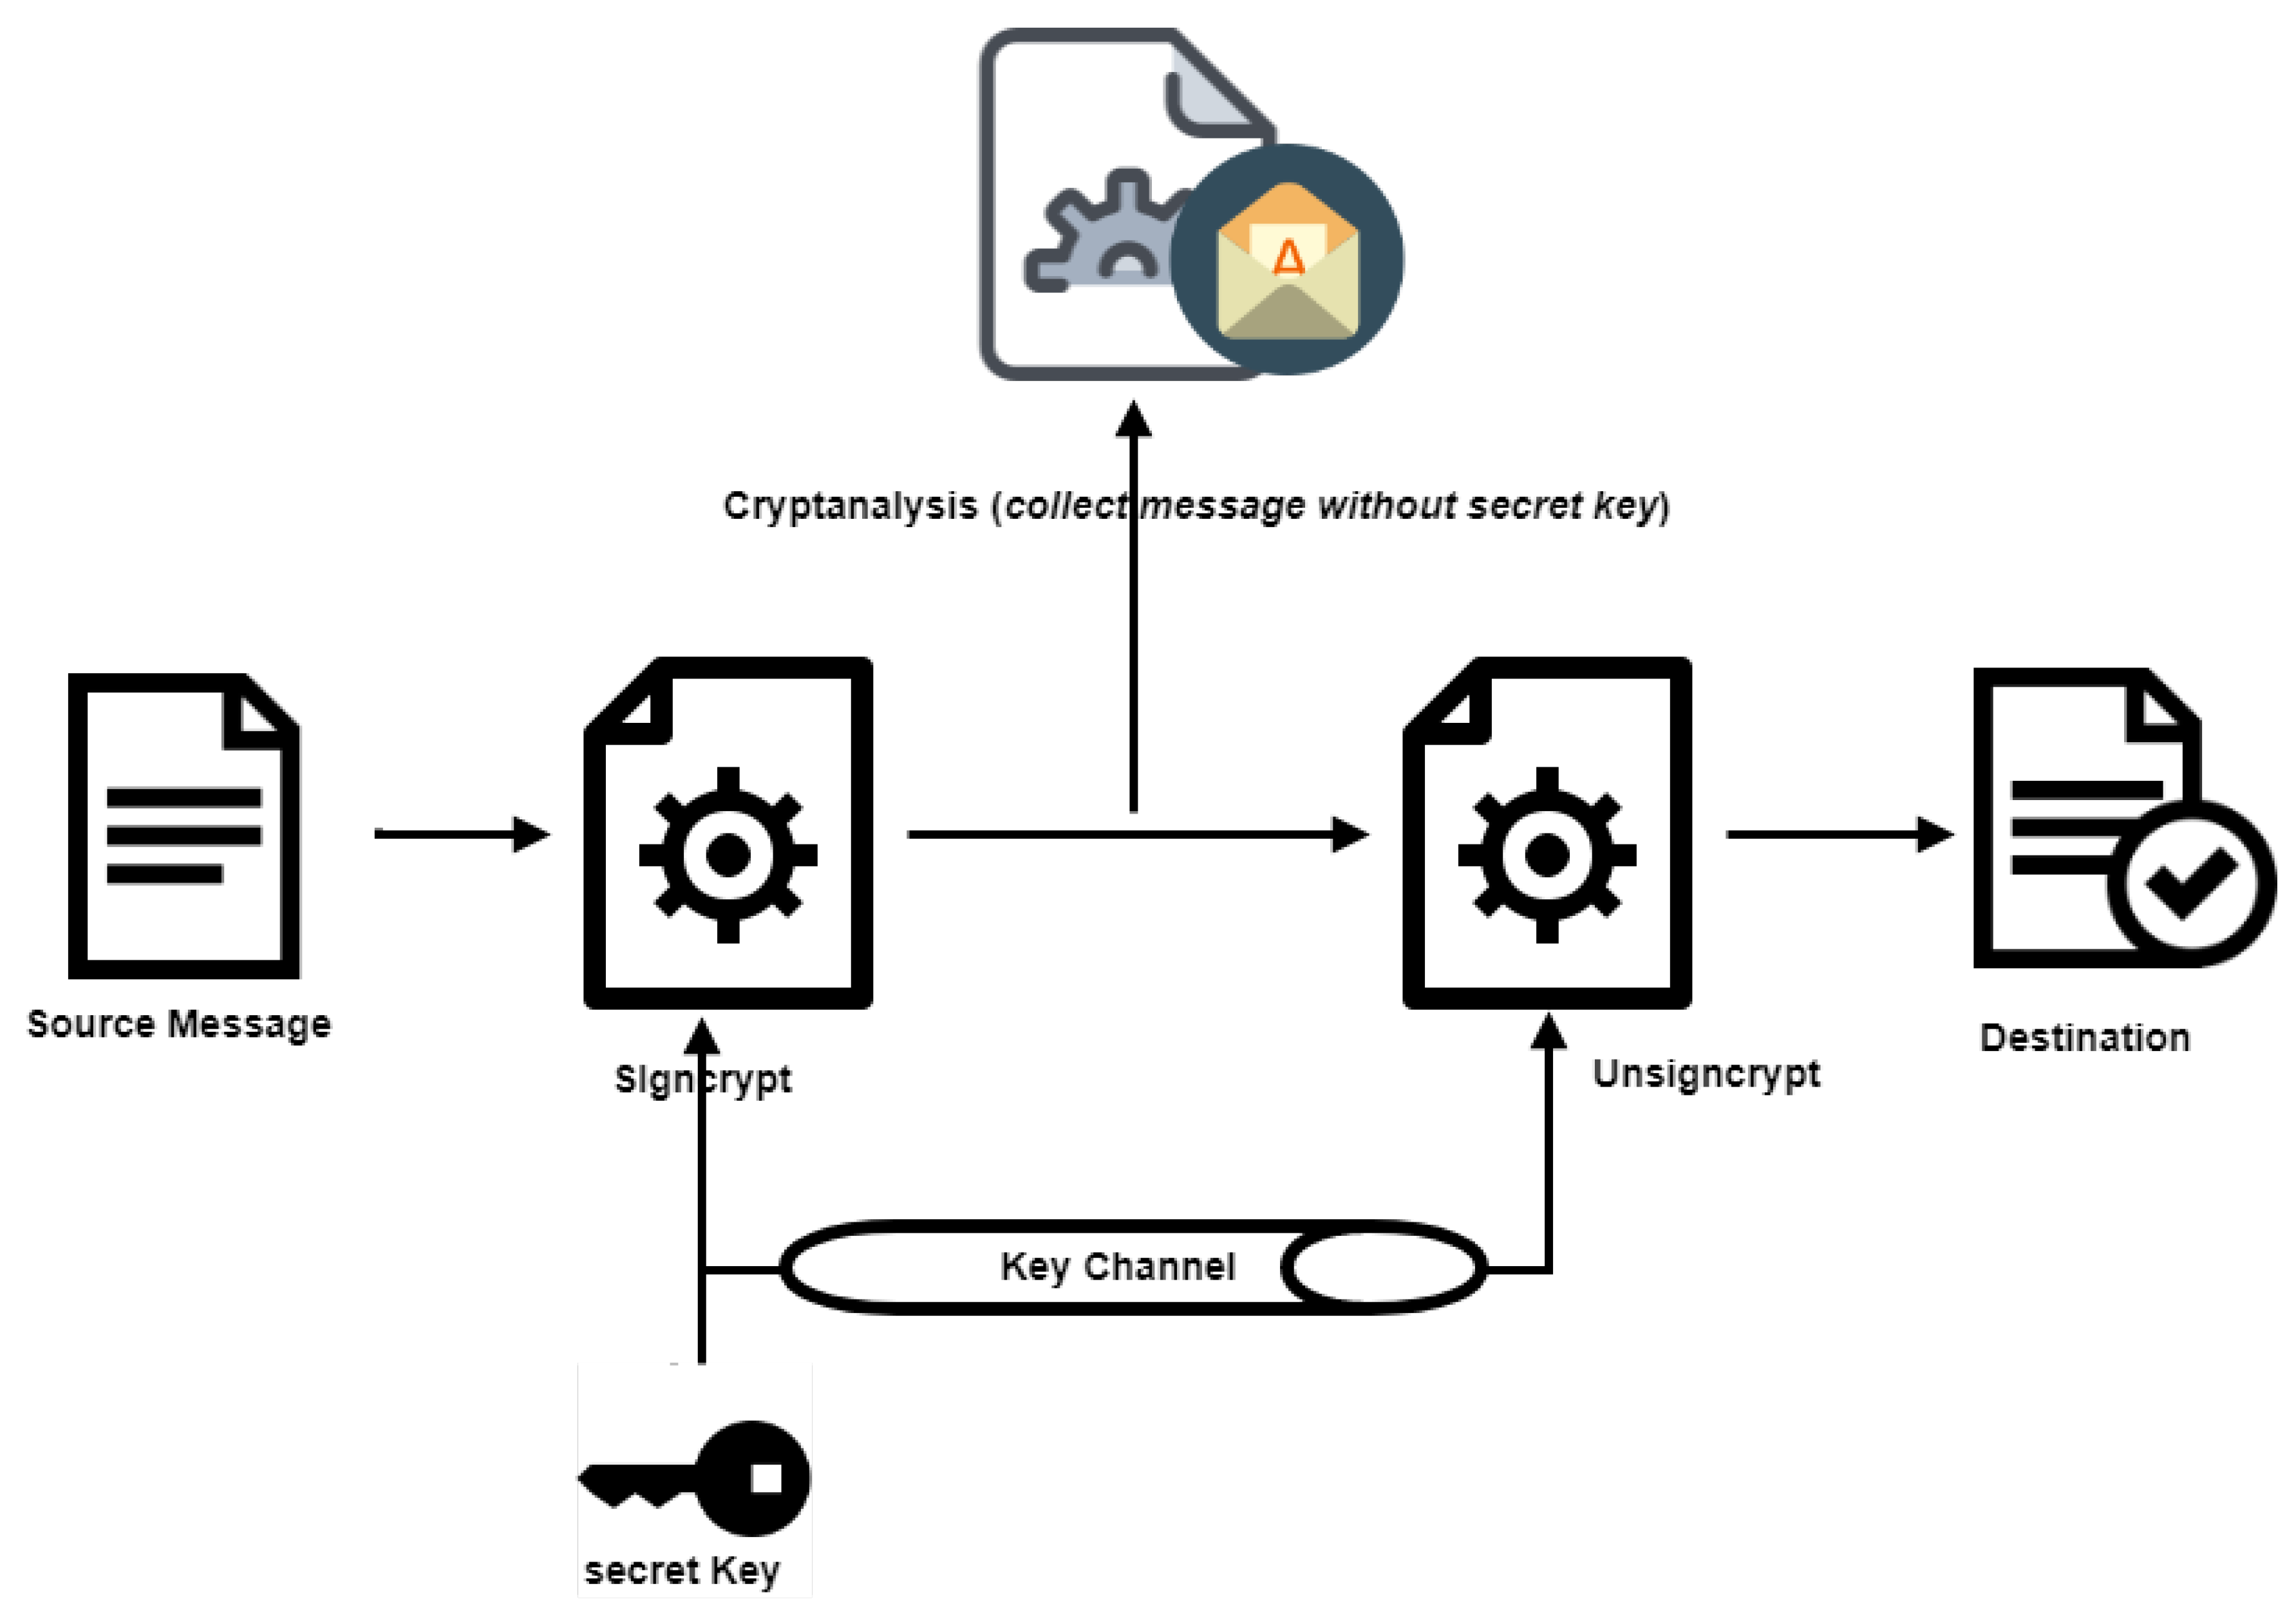
\includegraphics[scale=0.45]{imagenes/cryimage.png}
	\caption{Cryptanalysis cipher text}
\end{figure}

\subsection{CLASSIFICATION OF ATTACKS}

The main goal of a cryptanalyst is to obtain maximum
information about the plaintext (original data).Classification
of attacks can be done on following basis \cite{stallings2006cryptography}:
\begin{enumerate}
    \item{\textbf{Cipher text only attacks:} This is the most powerful attack. The
    attacker has only the knowledge of cipher text. This type of attack is
    successful only on the weakest of the ciphers.}
    \item{\textbf{Known plaintext attack:}attacker has the knowledge of plaintext and the corresponding cipher text, e.g. if an attacker is eavesdropping then  he can also guess the plaintext corresponding to some cipher texts depending upon the position or state of communication, in other words,  In this type a cryptanalyst have plaintext and their corresponding cipher text . Attacker tries to find out the relation between these two.}
    \item{\textbf{Chosen plaintext:}the attacker can choose its plaintext and get the cipher text corresponding to those chosen cipher text or The attacker obtain the various ciphertext corresponding to an arbitrary set of plaintext. }
    \item{\textbf{Chosen cipher text:} attacker is able to get the decrypted plaintext
    corresponding to his choice of cipher text. This attack is same as the
    chosen plaintext, but in a reverse direction which means The attacker obtain the various
    plaintext corresponding to an arbitrary set of cipher text}
    \item{\textbf{Adaptive chosen plaintext:}attacker first observes a large number of cipher texts. Based on the distribution of the cipher texts the attacker chooses a plaintext to get the corresponding cipher text which means the attacker chooses
    subsequent set of plaintext which is based on the information
    obtain from previous encryption methods.}
    \item{\textbf{Related Key: } This is a relatively new attack model. Here the attacker
    can encrypt two plaintext (same plaintext or the two plaintexts with a
    constant difference) with two keys, which have a fixed relation Between each other. This attack model is very weak as there is very little
    chance for the attacker to get encryption with two keys with a Constant
    relation. For lightweight block ciphers as the key is written to the device,
    this type of attack is not very probable.}
\end{enumerate}
\newpage
\subsection{Cryptanalytic technique}
In this section we will explain various cryptanalytic technique. As said earlier that, there are no fixed methods for cryptanalytic techniques for any block ciphers. But there are some methods which can be applied to every ciphers with some variation, though there can not be any guarantee that these methods may break the cipher. Cipher designers apply these methods to analyze security level for the computational security. Informally, broadly classify these techniques as brute force techniques non-brute force techniques. As the name suggest brute force techniques involves search of entire key space. Other techniques utilize the weakness in the structure of the ciphers to find key bits \cite{jha2011cryptanalysis}.

\subsubsection{Brute force technique:}
A brute-force attack is a can be used to attempt to decrypt any
encrypted data. Such an attack might be used when it is not possible to take
advantage of other weaknesses in an encryption system (if any exist) that
would make the task easier. When password guessing, this method is very
fast when used to check all short passwords, but for longer passwords other
methods such as the dictionary attack are used because a brute-force search
takes too long. Longer passwords, passphrases and keys have more
possible values, making them exponentially more difficult to crack than
shorter ones. can be made less effective by obfuscating the data to be
encoded making it more difficult for an attacker to recognize when the code
has been cracked or by making the attacker do more work to test each guess \cite{jha2011cryptanalysis}.

\subsubsection{Non-brute force techniques:}
In a non-brute-force attack, a single (usually common) password is
tested against multiple usernames or encrypted files. The process may be
repeated for a select few passwords. In such a strategy, the attacker is
Generally not targeting a specific user. Non brute-force attacks can be
mitigated by establishing a password policy that disallows common
passwords \cite{jha2011cryptanalysis}.
\newpage
\section{CipherText}
Ciphertext is encrypted text transformed from plaintext using an encryption algorithm. Ciphertext can't be read until it has been converted into  plaintext (decrypted) with a key. The decryption cipher is an algorithm that transforms the ciphertext back into plaintext.
The term cipher is sometimes used as a synonym for ciphertext. However, it refers to the method of encryption rather than the result.

\subsection{Types of ciphers}
There are various types of ciphers but We are focusing on only two of them that related to the work done , including:

\subsubsection{Transposition Cipher}
The transposition cipher is rearranged (change position only) the characters in the message but not change the characters. Transposition cipher have a pool of keys and ciphertext that rearranged the ciphertext for M times depended on the pool of keys. The output of transposition cipher saved in array of M locations we can called it \textit{plaintextArray}.
A simple transposition or permutation cipher works by breaking a message into fixed size blocks, and then permuting the characters within each block according to a fixed permutation, say P. The key to the transposition cipher is simply the permutation P. So, the transposition cipher has the property that the encrypted message contains all the characters that were in the plaintext message. In other words, the unigram statistics for the message are unchanged by the encryption process. The size of the permutation is known as the period. Let's consider an example of a transposition cipher with a period of ten 10, and a key P={7,10,4,2,8,1,5,9,6,3}. In this case, the message is broken into blocks of ten characters, and after encryption the seventh character in the block will be moved to position 1, the tenth moved character in the block will be moved to position 2, the forth is moved to position 3, the second to position 4, the eighth to position 5, the first to position 6, the fifth to the position 7, the ninth to the position 8, the sixth to the position 9 and the third to position 10.

In Table \ref{table:1} shows the key and the encryption process of the previously described transposition cipher. It can be noticed that the random string "X" was appended to the end of the message to enforce a message length, which is a multiple of the block size.It is also clear that thedecryption can be achieved by following the same process as encryption using the "inverse" of the encryption permutation. In this case the decryption key, P-1 is equal to {6,4,10,3,7,9,1,5, 8,2}.

\begin{table}[H]
    \begin{tabular}{|
    >{\columncolor[HTML]{FFFFFF}}l |}
    \hline
    \textbf{Key:}                                                                                                                                                                                  \\ \hline
    \begin{tabular}[c]{@{}l@{}}PlainText:    1 2 3 4 5 6 7 8 9 10\\ CipherText: 7   10 4 2 8 1 5 9 6 3\end{tabular}                                                                                \\ \hline
    \textbf{Encryption:}                                                                                                                                                                           \\ \hline
    \begin{tabular}[c]{@{}l@{}}Position:       123456789\textbf{10} 123456789\textbf{10}  123456789\textbf{10}\\ PlainText:    TRAISPNSTOIONROL\_AIGTHMXXXXXXX   \\ CipherText: OTNRSTSIPAGI\_OOIARLNXXXHXTXXXM\end{tabular} \\ \hline
    \end{tabular}
    \label{table:1}
    \caption{Encryption example of Transposition Cipher.}
    \end{table}
\newpage
\subsubsection{Substitution Cipher}
A cipher is an algorithm for encrypting plain text into cipher text and vice versa. The substitution cipher replaces every instance of a particular letter in the plain text with a different letter from the cipher text. Thus a substitution cipher key can be defined as the set of one-to-one mappings relating every letter in the plain text alphabet with the corresponding letter in cipher text alphabet. Such a key is normally defined using a table \ref{table:2}  and an example key is included below.
\begin{table}[h!]
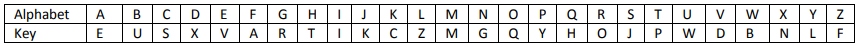
\includegraphics[width=0.9\textwidth]{imagenes/substitustion.png}\\
\caption{Substitution Cipher Example}
\label{table:2}
\end{table}

Thus the \textit{\textbf{HERE THE UNIVERSITY OF GRANADA}} can be encrypted to \textit{\textbf{QVOV PQV WGIDVOJPL QA ROEGEXE}},On the surface this cipher seems to be a strong one since there are 26 possibilities to choose from for the
first letter, 25 for the second, 24 for the third and so on. One can clearly see that there are in fact 26!
possible keys. 

\begin{equation} 26!= 26 * 25 * 24 * … * 1 = 4.03^{26} \end{equation}

However this cipher is particularly vulnerable to a technique known as frequency analysis since although it
does change the letters in the plain text to different ones in the cipher text it does not change the
underlying frequency of those letters.
Thus by comparing the frequencies of letters in the cipher text to a table of known letter frequencies for
the plain text language the key space can be reduced drastically. Furthermore you can also group letters
into n-grams where n represents the number of letters in the n-gram and look up the corresponding
frequencies for those \cite{brownbridge2007decrypting}. 
\newpage
\section{Genetic Algorithm}
Nature has always been a great source of inspiration to all mankind. Genetic Algorithms (GAs) are search based algorithms based on the concepts of natural selection and genetics. GAs are a subset of a much larger branch of computation known as Evolutionary Computation\cite{GAs}.
GAs were developed by John Holland and his students and colleagues at the University of Michigan, most notably David E. Goldberg and has since been tried on various optimization problems with a high degree of success\cite{GAs}.

The genetic algorithm is a general method of solving problems to
which no satisfactory, obvious, solution exists. It is based on the idea of
emulating the evolution of a species in nature, so the various components
of the Algorithm are roughly analogous to aspects of natural evolution.
Common mathematical tasks amenable to genetic solutions include
computing a curve to fit a set of data. Often these operators consist of
flipping a single.
Random bit of one individual or swapping two randomly selected
substrings from a pair of parents to generate a new child. To simulate
Darwinian survival of the fittest some representation of the fitness of the
individuals must be generated \cite{toemeh2007breaking}.

Genetic Algorithm Attack is more complicated than the  any other attack. This is because a pool of solutions is being maintained, rather than a single solution.
An extra level of complexity is also present because of the
need for a mating function and for a mutation function \cite{dimovski2003attacks}.

Genetic Algorithms are sufficiently randomized in nature, but they perform much better than random local search (in which we just try various random solutions, keeping track of the best so far), as they exploit historical information as well \cite{GAs}.
\newpage
\subsection{The steps of the genetic algorithm}
The genetic Algorithm has six steps which can evolve solutions to the search problem the following \cite{sastry2005genetic}:
\subsubsection{Initialization(Population)}
The initial population of candidate solutions is usually generated
randomly across the search space. However, domain-specific knowledge or other
information can be easily incorporated in the generation of the initial population.
The population is usually defined as a two dimensional array of size population, size x , chromosome size.
There are two primary methods to initialize a population in a GA. They are:
\subsubsection{Random Initialization:} Populate the initial population with completely random solutions.
\subsubsection{Heuristic initialization:} Populate the initial population using a known heuristic for the problem

\subsubsection{Evaluation(Fitness):}
Once the population is initialized, or an offspring population is created, the fitness values of the candidate solutions are evaluated.
A fitness function should possess the following characteristics:
\begin{enumerate}
    \item{The fitness function should be sufficiently fast to compute.}
    \item{It must quantitatively measure how fit a given solution is or how fit individuals can be produced from the given solution.}
\end{enumerate}

\subsubsection{Selection:} 
Selection allocates more copies to solutions with better fitness values and thus imposes the survival-of-the-fittest mechanism on the candidate solutions. The main idea of selection is to prefer better solutions to worse ones, and many selection procedures have been proposed to accomplish this idea, 
\subsubsection{Recombination(Crossover):}
Recombination combines bits and pieces of two or more parental solutions to create new, possibly better solutions (i.e. offspring). There are many ways of accomplishing this, and achieving competent performance depends on getting the recombination mechanism designed properly; but the primary idea to keep in mind is
that the offspring under recombination will not be identical to any particular parent and will instead combine parental traits in a novel manner \cite{goldberg1999using}.
\newpage
In GAs a crossover can be of following operators:
\subsubsection{Single Point Crossover:}
In this one-point crossover, a random crossover point is selected and the tails of its two parents are swapped to get new off-springs, as shown in figure \ref{onePointfigure}.

\begin{figure}[h]
	\centering
	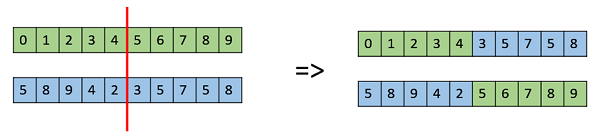
\includegraphics[scale=0.45]{imagenes/one_point_crossover.png}
    \caption{One Point Crossover operator}
    \label{onePointfigure}
\end{figure}

\subsubsection{Multi Point Crossover:}
Multi point crossover is a generalization of the one-point crossover wherein alternating segments are swapped to get new off-springs, as shown in figure \ref{MultiPointfigure}

\begin{figure}[h]
	\centering
	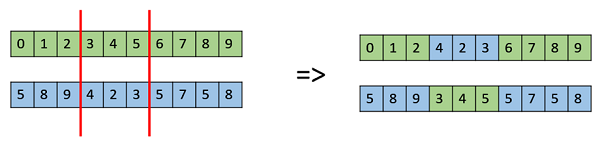
\includegraphics[scale=0.45]{imagenes/multi_point_crossover.png}
    \caption{Multi Point Crossover operator}
    \label{MultiPointfigure}
\end{figure}

\subsubsection{Uniform Crossover:}
In a uniform crossover, we don’t divide the chromosome into segments, rather we treat each gene separately. In this, we essentially flip a coin for each chromosome to decide whether or not it’ll be included in the off-spring. We can also bias the coin to one parent, to have more genetic material in the child from that parent, as shown in figure \ref{uniformfigure}.

\begin{figure}[h]
	\centering
	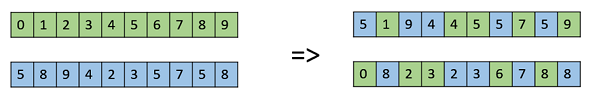
\includegraphics[scale=0.45]{imagenes/uniform_crossover.png}
    \caption{Uniform Crossover operator}
    \label{uniform}
\end{figure}

\subsubsection{Mutation:}
While recombination operates on two or more parental chromosomes,
mutation, locally but randomly, modifies a solution. Again, there are many variations of mutation, but it usually involves one or more changes that are made to
an individual’s trait or traits. In other words, mutation performs a random walk
in the vicinity of a candidate solution, as shown in figure \ref{mutation}.

\begin{figure}[h]
	\centering
	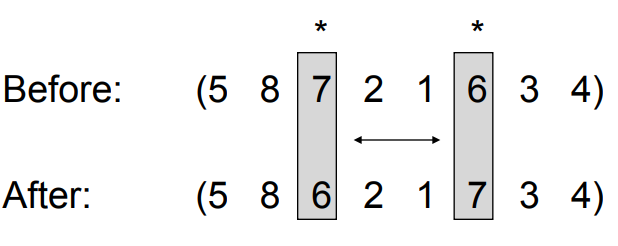
\includegraphics[scale=0.45]{imagenes/mutation.png}
    \caption{Mutation Example}
    \label{mutation}
\end{figure}

\subsubsection{Replacement:}
The offspring population created by selection,
recombination, and mutation replaces the original parental population.
Many replacement techniques such as elitist replacement, generationwise replacement and steady-state replacement methods are used in
GAs.

\subsection{Advantages and Limitations of Genetic Algorithms}
\subsubsection{Advantages}
GAs have various advantages which have made them immensely popular. These include:
\begin{enumerate}
    \item{Does not require any derivative information (which may not be available for many real-world problems).}
    \item{Is faster and more efficient as compared to the traditional methods.}
    \item{Has very good parallel capabilities.}
    \item{Optimizes both continuous and discrete functions and also multi-objective problems.}
    \item{Provides a list of “good” solutions and not just a single solution.}
    \item{Always gets an answer to the problem, which gets better over the time.}
    \item{Useful when the search space is very large and there are a large number of parameters involved.}
\end{enumerate}
\subsubsection{Limitations}
Like any technique, GAs also suffer from a few limitations. These include:
\begin{enumerate}
    \item{GAs are not suited for all problems, especially problems which are simple and for which derivative information is available.}
    \item{Fitness value is calculated repeatedly which might be computationally expensive for some problems.}
    \item{Being stochastic, there are no guarantees on the optimality or the quality of the solution.}
    \item{If not implemented properly, the GA may not converge to the optimal solution.}
\end{enumerate}

\subsection{Application areas of genetic algorithm (GA):}
Genetic Algorithms are primarily used in optimization problems of
various kinds, but they are frequently used in other application areas as
well. Some of the areas in which Genetic Algorithms are frequently used
explained in the following:
\subsubsection{Optimization:}
Genetic Algorithms are most commonly used in
optimization problems wherein we have to maximize or minimize.
Given objective function value under a given set of constraints. The
approach to solve Optimization problems has been highlighted
throughout the tutorial. 
\subsubsection{Economics:}
GAs are also used to characterize various economic
models like the cobweb model, game theory equilibrium resolution,
asset pricing, etc.
\subsubsection{Parallelization:}GAs also have very good parallel capabilities, and
prove to be very effective means in solving certain problems, and
provide a good area for research.
\subsubsection{Image Processing:} GAs are used for various digital image processing
(DIP) tasks as well like dense pixel matching.
\subsubsection{Vehicle routing problems:} With multiple soft time windows, multiple
depots and a heterogeneous fleet.
\subsubsection{Scheduling applications:}GAs are used to solve various scheduling
problems as well, particularly the time tabling problem.
\subsubsection{Machine Learning:}genetics based machine learning (GBML) is a
niche area in machine learning
\subsubsection{Robot Trajectory Generation:}GAs have been used to plan the path
which a robot arm takes by moving from one point to another.
\subsubsection{Parametric Design of Aircraft:}GAs have been used to design
aircrafts by varying the parameters and evolving better solutions.
\newpage

